

\documentclass[10pt, conference, compsocconf]{IEEEtran}

\usepackage{color,soul}
\usepackage{listings}
\usepackage{hyperref}
\usepackage{blindtext}
 \usepackage{graphicx}
\lstset{basicstyle=\footnotesize\ttfamily,breaklines=true}
\lstset{frame=lines}

\ifCLASSINFOpdf
  % \usepackage[pdftex]{graphicx}
  % declare the path(s) where your graphic files are
  % \graphicspath{{../pdf/}{../jpeg/}}
  % and their extensions so you won't have to specify these with
  % every instance of \includegraphics
  % \DeclareGraphicsExtensions{.pdf,.jpeg,.png}
\else
  % or other class option (dvipsone, dvipdf, if not using dvips). graphicx
  % will default to the driver specified in the system graphics.cfg if no
  % driver is specified.
  % \usepackage[dvips]{graphicx}
  % declare the path(s) where your graphic files are
  % \graphicspath{{../eps/}}
  % and their extensions so you won't have to specify these with
  % every instance of \includegraphics
  % \DeclareGraphicsExtensions{.eps}
\fi



% correct bad hyphenation here
\hyphenation{op-tical net-works semi-conduc-tor}

\graphicspath{{figures/}}



\begin{document}
%
% paper title
% can use linebreaks \\ within to get better formatting as desired
\title{SamzaSQL: Open Source Distributed Fast Data Management System}


% author names and affiliations
% use a multiple column layout for up to two different
% affiliations

% \author{\IEEEauthorblockN{Milinda Pathirage\IEEEauthorrefmark{1} and
% Beth Plale\IEEEauthorrefmark{2}}
% \IEEEauthorblockA{School of Informatics and Computing,
% Indiana University\\
% Email: \IEEEauthorrefmark{1}mpathira@indiana.edu,
% \IEEEauthorrefmark{2}plale@cs.indiana.edu}
% \and
% \IEEEauthorblockN{Yi Pan\IEEEauthorrefmark{3} and
% Chris Riccomini \IEEEauthorrefmark{4}}
% \IEEEauthorblockA{LinkedIn\\
% Email: \IEEEauthorrefmark{3}yipan@linkedin.com,
% \IEEEauthorrefmark{4}criccomini@linkedin.com}
% \and
% \IEEEauthorblockN{Julian Hyde\IEEEauthorrefmark{5}}
% \IEEEauthorblockA{Hortonworks\\
% Email: \IEEEauthorrefmark{5}julian@hydromatic.net}
% }

\author{
    \IEEEauthorblockN{Milinda Pathirage\IEEEauthorrefmark{1}, Yi Pan\IEEEauthorrefmark{2}, Chris Riccomini\IEEEauthorrefmark{2}, Julian Hyde\IEEEauthorrefmark{3} and Beth Plale\IEEEauthorrefmark{1}}
    \IEEEauthorblockA{\IEEEauthorrefmark{1}School of Informatics and Computing, Indiana University
    \\\{mpathira, plale\}@indiana.edu}
    \IEEEauthorblockA{\IEEEauthorrefmark{2}LinkedIn
    \\\{yipan, criccomini\}@linkedin.com}
    \IEEEauthorblockA{\IEEEauthorrefmark{2}Hortonworks
    \\julian@hydromatic.net}
}

% make the title area
\maketitle


\begin{abstract}
In a data-driven economy, it's important act on data as it arrives to stay competitive. Specialized message queues like Kafka and specialized streaming processing platforms like Apache Samza was invented to take value out of fast data. But these system still lacks support for standard querying capabilities which is available in \textit{Big Data} processing systems like \textit{Hive} or \textit{Presto}. In this paper, we describe a SQL based streaming data querying and manipulation framework implemented on top of Apache Samza -- a open source stream processing framework.
\end{abstract}

\begin{IEEEkeywords}
Big Data; SQL; Streaming;

\end{IEEEkeywords}


% For peer review papers, you can put extra information on the cover
% page as needed:
% \ifCLASSOPTIONpeerreview
% \begin{center} \bfseries EDICS Category: 3-BBND \end{center}
% \fi
%
% For peerreview papers, this IEEEtran command inserts a page break and
% creates the second title. It will be ignored for other modes.
\IEEEpeerreviewmaketitle



\section{Introduction}
In today’s data-driven economy, enterprises – whether \textit{big} or \textit{small} – depends on data analytics to provide better services as well as to carry out most of the day to day business functions. Driven by unprecedented growth of \textit{mobile} and \textit{Internet of Things} (IoT) related technologies, ever increasing rate of data growth has changed how enterprises manage and interact of data. As a result \textit{Big Data} related technologies such as Hadoop became accessible to broad spectrum of users -- from small to big enterprises -- enabling analysis of petabytes of data on commodity clusters.

Often these massive quantities of data is created by events occuring thousands to tens of thousands of times per second as a result of web interactions, remote sensors reacting to change of environment, etc. With these data generation rates we not only talks about \textit{volume} of data, we also talks about \textit{velocity} of data. And as the data-driven economy evolves, enterprises also realized the importance of interacting with the data (raw events) as it arrives to create new business oppertunities. 

Couple of years ago, it was impracticle to act on high volumes of data as it arrives due to higher latencies of Big Data processing tools and cost of specialized software and hardware. As a result, distributed message queues and stream processing systems like \textit{Apache Kafka}, \textit{Apache S4}, \textit{Apache Storm} and \textit{Apache Samza} which are robust and scalable enough to handle massive volumes of fast moving data were invented. These systems allows us to act on data as it arrives, generating value to both organisations and its users.

As people realize the value of data in motion is equal or greater than the data at rest, new scalable and fault-tolerant data management architectures such as \textit{Lambda Architecture (LA)} was proposed tackle wide range of requirements from low latency analytics to high latency analytics. Lambda architecture consists of three main layers -- speed layer, batch layer and serving layer -- where speed layer process data in motion and batch layer process data at rest while serving layer provide querying mechanism on top of results generated by speed layer and batch layer.  While there are several imlementaitons of LA \cite{boykin2014summingbird} \cite{metamarkets:radstack}, opponents of Lambda Architecture argued \cite{questions-la-kreps} that its possible to achieve same using only a stream processing system by retaining the input data unchanged as proposed in LA and reprocessing by increasing the parallelism and replaying historical data as fast as possible. The main advantage of this new way of processing data is that you don't have to manage two entirely different systems (a batch processing system such as Hadoop and stream processing system such as Storm or Samza). Fernandez et al. recently presented in \cite{fernandezliquid} an improved version of this new architecture deployed at LinkedIn which is built on top of Apache Samza and Apache Kafka.  

Instead of widely used and standard declarative language like SQL, implementations of architectures mentioned above provide APIs in high level languages like Java \cite{samza:api} or Scala \cite{boykin2014summingbird} or custom query languages \cite{metamarkets:radstack} specific for the framework. Also our experience with Lambda architecture framework like \cite{boykin2014summingbird} shows that understanding of complex programming abstractions are required to take the advantage of these frameworks. But custom programs written for specific purposes add maintenance overhead and often hard to reuse. And custom query languages doesn't have the advantages of extensions (for stream processing specific scenarios) to standard SQL such as

\begin{itemize}
  \item easy to learn if you know SQL
  \item clear semantics
\end{itemize}

In this paper, we present \textit{SamzaSQL}, scalable and fault-tolerant open-source SQL based streaming query engine implementation with support for interacting with non-streaming data sources on top of Apache Samza. Wide adoption of Hive and Drill like frameworks to query Big Data is a good indicator for requirement of SQL based analytics for fast data and in this work we try to provide similar capabilities provided by Hive for Big Data to fast data analytics using Samza SQL. We believe that providing DBMS like capabilities over fast data streams will make it easy to realize Kappa architecture style solutions and we also envision that SQL compliant fast data management system will make fast data analytics accessible to broad community of users because they can utilize knowledge of SQL in the context of fast data analytics.

SamzaSQL supports queries expressed in standard SQL with minor extensions to add stream producing and windowing capabilities. These queries get compiled into streaming jobs executed in Samza. Depending on the query, these streaming jobs may involve access to static data sources such as stored relations and may access outputs from recurring high latency jobs. SamzaSQL front-end, which does query parsing, validation and planning is built on top of \textit{Apache Calcite} and supports querying stream data formats such as Avro or JSON. SamzaSQL also includes support for pluggable schema catalogs enabling integration of different data formats and stores. Windowing is a core and central concept of stream querying due to the fact that operators like \textit{join} and some of the aggregations cannot be evaluated over unbounded streams. SamzaSQL comes with a widow operator implementation with supports for 

\begin{itemize}
\item timely and deterministic window output under unpredictable message delevery latencies
\item and, deterministic window output with node failures and message re-delivery
\end{itemize}

Until now, we have used custom programs or data processing pipelines built on APIs provided by streaming and batch data processing frameworks or programming models such as Summingbird \cite{boykin2014summingbird} to build Lambda or Kappa architecture style applications. General motivation of this work is to explore how we can provide a unified framework -- which enables Kappa architecture style data processing pipelines based on well known standard SQL. Also its worth noting that Samza SQL supports nearline analytics tasks with latency requirements in the order of seconds and replaying based high latency tasks with latencies in the order of minutes or hours.

Our main contributions are:

\begin{itemize}
  \item Streaming SQL implementation of Samza
\end{itemize}


Rest of the paper is organised as follows. In Section \ref{sec:overview} we provide a system overview including important requirments with a sample application. Then, in Section \ref{sec:design} we discussed system architecture and reasoning behind different design decisions made. Section (TODO) describes the SamzaSQL implementation. Then in Section (TODO) we evalute SamzaSQL based application development experience against vanila Samza application development and we also do a performance study comparing Samza SQL and vanilla Samza based streaming tasks. In Section (TODO), we discuss some of the interesting related work in the context of SamzaSQL. Finally in the Section (TODO), we conclude the paper with our findings and experience.

\section{System Overview with Example}
\label{sec:overview}
Consider a stream of ad click events, where events are encoded in Avro format with the schema:

\begin{lstlisting}
{
     "type": "record",
     "namespace": "org.apache.samza",
     "name": "AdClick",
     "fields": [
       { "name": "clickTime", "type": "long" },
       { "name": "userId", "type": "long"},
       { "name": "adId", "type": "long"}
     ]
}
\end{lstlisting}

User wants to compute, for each ad, a 5-minute windowed count of clicks on that ad, across a 5% sample of users in near realtime.

\subsection{User Experience}
Its theoritically possible to using any type of messaging system to input data streams to Samza. But Kafka is the preffered and stable messaging infrastructure for Samza. Lets assume 

\begin{itemize}
  \item events are published to a Kafka topic \textit{adclick}, partitioned on adId
  \item \textit{adclick} topic is registered in a Kafka \textit{Schema Registry} instance known to the Samza SQL query driver
\end{itemize}

When connected to a Kafka Schema Registry instance, Samza SQL driver automatically lazy loads stream definitions into the query planner's in-memory metadata store and topic registered in that instance of Schema Registry instance will be visible to the query planner with correct type informations. So the user can write the above mentioned  query logic as a Samza SQL query:

\begin{lstlisting}[language=SQL]
SELECT STREAM 
  round5min(clickTime to timestamp) as clickTime,
  COUNT(*) as clicks
FROM adclick
WHERE userId % 100 < 5
GROUP BY round5min(clickTime to timestamp), adId;
 \end{lstlisting}

\begin{table}
\centering
\setlength\tabcolsep{4pt}
\begin{minipage}{0.2\textwidth}
\centering
\begin{tabular}{ |c|c|c| } 
\hline
clickTime & userId & addId \\
\hline
10:00:00  & 30 & 2 \\
10:02:43  & 10 & 1 \\
10:04:23  & 20 & 1 \\
10:06:10  & 10 & 3 \\ 
10:04:56  & 40 & 2 \\  
\hline
\end{tabular}
\caption{Input Stream}
\label{tab:input} 
\end{minipage}%
\hfill
\begin{minipage}{0.2\textwidth}
\centering
\begin{tabular}{ |c|c|c| } 
\hline
clickTime & userId & addId \\
\hline
10:00:00  & 30 & 2 \\
10:02:43  & 10 & 1 \\
10:04:23  & 20 & 1 \\
10:06:10  & 10 & 3 \\ 
10:04:56  & 40 & 2 \\ 
\hline
\end{tabular}
 \caption{Output} 
 \label{tab:output} 
\end{minipage}
\end{table}


 The result of the above query will be a stream. At every 5-minutes Samza SQL will emit click count of ads with clicks in previous 5-minutes. Late arrivals will be handled according to the windowing policy and updated count will be emitted to the output stream. Samza SQL infer that it needs to emit ad click counts at every 5-minutes based on the fact that it knows \textit{clickTime} is increasing  and also knows that round5min(clickTime to timestamp) is also increasing. For example once Samza SQL sees a row at or after 10:05:00 it knows that, it needs to emit a patial ad click count for last 5 minutes and when there is a another ad click event belongs to 10:00:00 to 10:05:00 interval it will update previous count and re-emit the counts for that time period until window close timeout is passed. 

The columns or expressions that is increasing or decreasing is know as \textit{monotonic} column/expression. Without a monotonic expression in GROUP By query, Samza SQL can't make any progress in streaming queries and will throw a error at query validation phase. 

To handles aggregates like above, Samza SQL implements a relaxed version of SQL stream aggregation where rows can be out of order to accomodate late arrivals common in distributed data streams. Samza SQL window aggregates emit partial results as soon as possible and handle the out of order tuples according to windoing policy. For Samza SQL tumbling window aggregate like above, single input row can be contributed to multiple output rows due to partial aggregation which is completely different from standard SQL aggregate semantic where each input row contributes to only one output row.

If user wants this output stream to be appear in a another stream he can use INSERT INTO query to deliver the results of this query to an another stream.

\begin{lstlisting}[language=SQL]
INSERT INTO adclickcounts
  SELECT STREAM 
    round5min(clickTime to timestamp) as clickTime,
    COUNT(*) as clicks
  FROM adclick
  WHERE userId % 100 < 5
  GROUP BY round5min(clickTime to timestamp), adId;
\end{lstlisting}

Some other important use cases in a streaming query context are joining with stored relations and windowed joins. Samza SQL provide support for those constructs as well, but the full description on query implementation is outside the scope of this paper. But we note that Samza SQL supports all the basic standard SQL constructs on both streams and relations.

Samza SQL is quite different from existing systems which implements Lambda architecture and Kappa architecture mainly because Samza SQL is build based on relational algebra and it views streams as relations that varies with time similar to CQL. This enabled easy integration of slow-changing data into streaming queries as well as provides consistent view across both streaming and relational data sources.

\subsection{System Overview}

Samza SQL first compile user query into a logical query plan and then optimize this logical query plan based on different heuristics and metrics related streaming. Then this logical query plan get converted into a physical plan consisting Samza SQL operator DAG. Each of these operators consume one or more streams of tuples and produces a stream of tuples where tuple represents a single stream element. Samza pulls tuples from input streams (sources) and push them to the operators. Elements in a stream can be formatted using a message format like Avro or JSON and Samza SQL provide plugging architecture to integrate new message formats to the framework. 

Samza SQL supports queries on both streams and tables where

\begin{itemize}
  \item A stream is a (possibly infinite) sequence of elements partitioned by user selected key or partitioning mechanism and a partition is an ordered, immutable sequence of elements.
  \item A table is analogous to tables in relational databases, but not limited only to relational databases. Samza SQL provides extension mechanisms necessary to support different types of slow-changing data sources based on user preference.
\end{itemize}

The output from streaming SQL queries can be ingested into an another stream or a database for further consumption. Query results can also be materialized into materialized views. Samza SQL encourage ingesting streaming outputs into an another stream for easily handling of partial aggregates caused by out of order arrival of data. Most important requirements and Samza SQL design decisions which caters those requirements are summarized below and discussed in the coming sections including a performance evaluation of current implementation.

\subsubsection{Familiar language}

Samza SQL uses extended version of standard SQL which makes it easy to learn for anyone who knows SQL. As a result this results in clear semantics where we try to produce same results on a stream as if the data were in a table. For example, Samza SQL produce same result for tumbling window query 1 if there aren't any out of order tuples. But in case of out of order tuples there can be multiple partial emits until window is closed. Also using extended version of standard SQL helped us to utilize existing query parsing and optimization framework in the front-end. This reduces development time as well as it gave us lot of opportunity focus on the streaming aspects of the system.

\subsubsection{Early results and incremental processing}

Its important to support incremental processing in streaming query engines. Samza SQL implements all the aggregations in incremental fashion and different window policies are employed to produce partial early results in the presence of out of order arrivals. Samza SQL detect queries of blocking nature early at the query validation phase to prevent accidental infinitely blocking queries during runtime.

\subsubsection{Support both streams and relations}

Samza SQL supports both streams and relations from slow-changing data sources like NoSQL storages and relational databases. We are utilizing Calcite capability to generate query plans consisting of scanning both streams and relations to implement this functionality for Samza SQL. This 

\subsubsection{Parallelism and Scalability}

Initial implementation of Samza SQL supports data parallelism using Kafka's partitioning capabilities. Each partition will be handled by Samza SQL task specific to that partition. Task parallelism for scaling large queries are not supported yet.

\subsubsection{Fault tolerance}

Samza SQL achieve fault tolerance using Samza's local storage and reply capability. Local state of Samza SQL tasks will be backed up as a change stream and in case of a failure tasks will get restored with local state containing data up to last know checkpoint. In addition to that Samza SQL will checkpoint window processing into a another change stream such that it can replay tuples lost due to task failure from Kafka after restoring the local state.

\subsubsection{Ability to replay}


\subsubsection{Materialized views}

\section{System Architecture}

In response to the challenges and requirements discussed in Section \ref{sec:overview}, we developed SamzaSQL, a scalable and fault-tolerant fast data query engine capable of supporting nearline analytics tasks, replay based offline analytics and quries with access to both streams and slow-changing stored relations. In this section, we outline the SamzaSQL architecture.

\begin{figure}[h!]
  \centering
  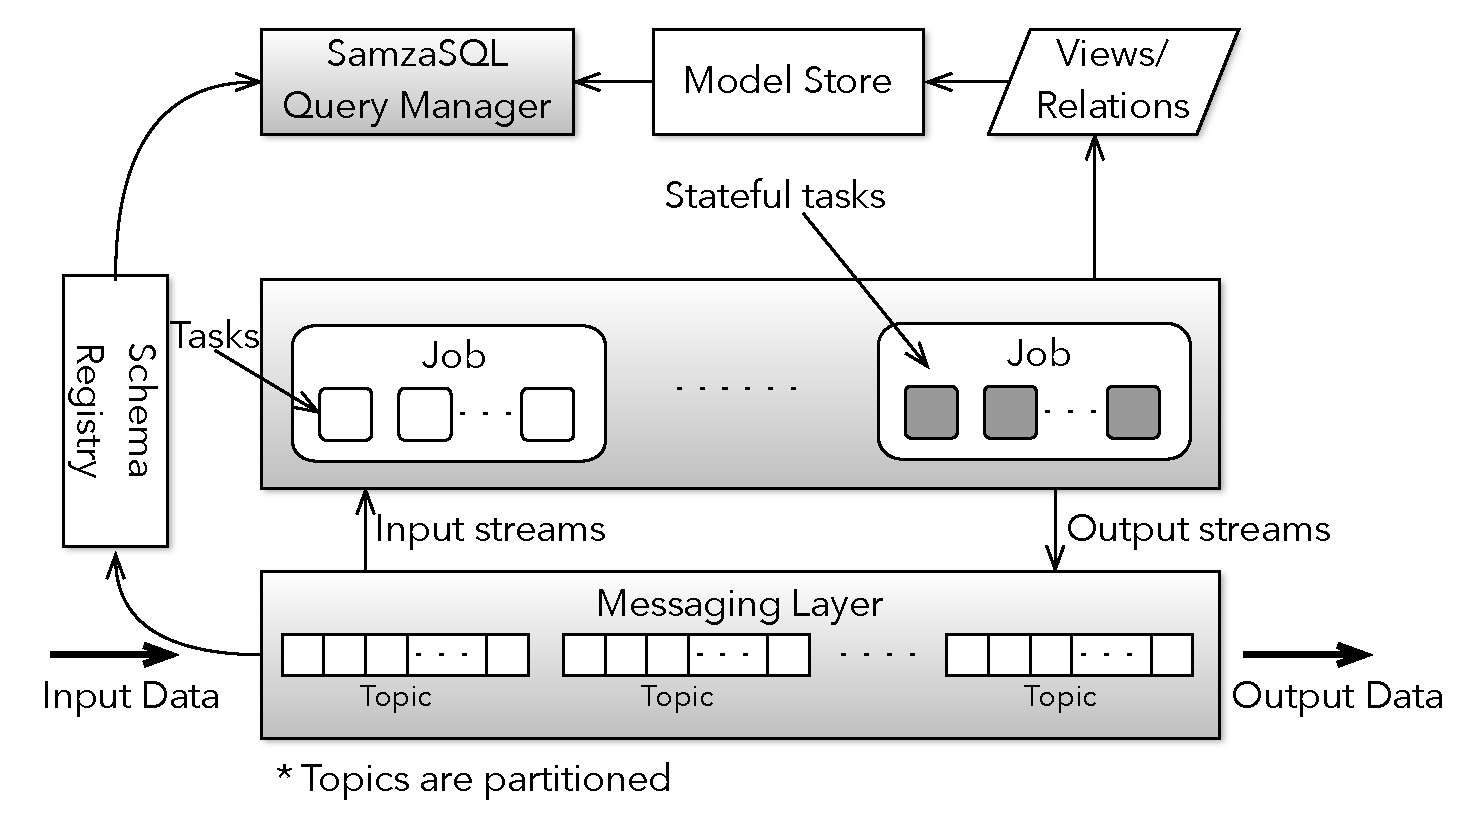
\includegraphics[width=0.5\textwidth]{samzasql-arch}
  \caption{\textbf{SamzaSQL Architecture} Three main components, Query Manager, Processing Layer and Messaging Layer. Processing layer backed by high-available messaging layer executes jobs submitted by query manager for user submitted streaming SQL queries.}
  \label{fig:arch}
\end{figure}

SamzaSQL consists of three primary architectural components colored dark in Figure \ref{fig:arch}. The \textbf{SamzaSQL query manager} accepts queries from users, deploys optimized jobs generated from the query and keeps track of queries and their respective jobs. In addition to that the query manager  provides a schema discovery (for both streams and relations) abstraction for query processor. 

The \textbf{processing layer} executes stateful streaming jobs for queries, handle scheduling of tasks for jobs, provides resource isolation and fault-tolerance, guarantees low latency processing, enables incremental processing and provides replayable data processing framework. SamzaSQL currently uses Apache Samza \cite{asf:2014:samza} as its processing engine due to stateful, fault-tolerant and replayable streaming processing model support by Samza. But its possible to replace Samza with different stream processing engine as long as it supports stateful processing model and replayable streams.

The \textbf{messaging layer} supports the processing layer by providing highly available storage for high-volume fast data (both inputs and outputs) and checkpointing and recovery information (for local state). Messaging layer also offers rewindability which enables replay based offline analytics and failure recovery. Current implementaiton of SamzaSQL uses Apache Kafka \cite{kreps2011kafka} distributed message queue for messaging layer. Samza natively supports Kafka and high-availability, scalability and stream rewindability features in Kafka enables most important features of Samza like checkpoint based local state recovery and replay based failure handling. 

SamzaSQL supports streaming and relational data sources via extendable schema factory and table scan abstraction. This allows SamzaSQL read/write data from/to any storage system that can be exposed to SamzaSQL as a relation via above mentioned abstractions allowing stream to relation joins and relational view materialization.

SamzaSQL achieves data parallelism by assigning one or more Kafka partitions to a task in Samza job and task parallelism by dividing a single query into multiple Samza jobs. Figure \ref{fig:parallelism} briefly visualize how SamzaSQL queries are parallelised for scalability.

\begin{figure}[h!]
  \centering
  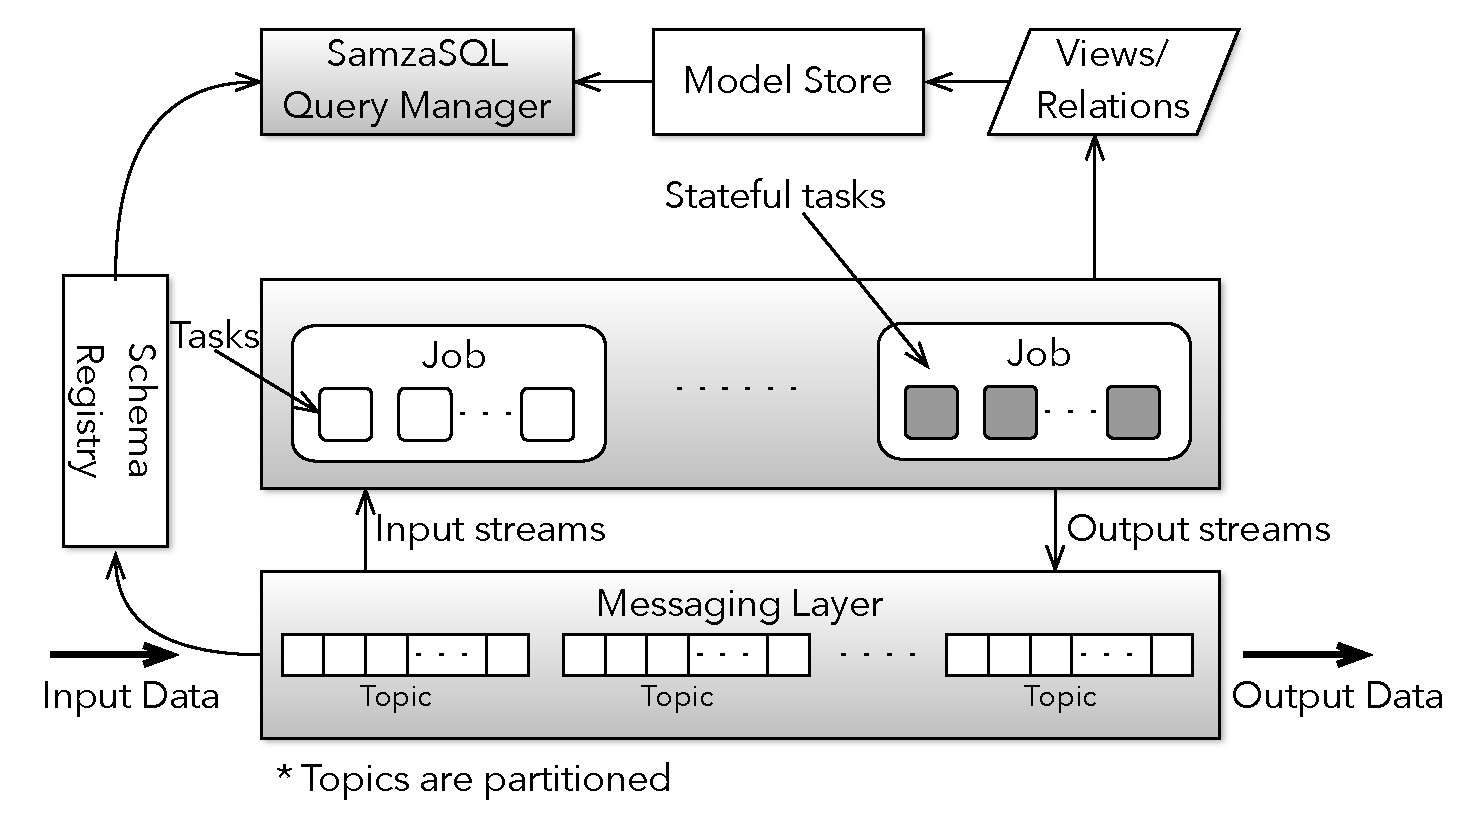
\includegraphics[width=0.5\textwidth]{samzasql-arch}
  \caption{\textbf{SamzaSQL Architecture} Three main components, Query Manager, Processing Layer and Messaging Layer. Processing layer backed by high-available messaging layer executes jobs submitted by query manager for user submitted streaming SQL queries.}
  \label{fig:parallelism}
\end{figure}

In coming sections, we provide greater detail about the SamzaSQL implementation and some of the design decisions behind the implementation. We also provide performance comparison between SamzaSQL queries and same queries implemented as native Samza jobs in Java in Section (TODO).



\section{Implementation}

\section{Evaluation}

\section{Related Work}

\section{Future Work}

\section{Conclusion}

\section{Acknowledgement}

The authors would like to thank Jay Kreps, Martin Kleppman, Navina Ramesh, Guzhang Wang; and the Apache Samza community for their valueable feedback.

\bibliographystyle{IEEEtran}
\bibliography{IEEEabrv,references}

% that's all folks
\end{document}


